\chapter{Computational modelling of tissue ablation}



%More background on why developing the laser ablation model. 
%What is the medical reason to want this. 
%What medical procedures are done with laser ablation? 
%What are the outstanding issues/questions that your model can be used to answer? mention pig skin

%Details of laser pulsing.
%Time steps, convergence tests, etc
%Time for holes to be drilled by laser.
%Low intensity damage
%in equation 9, could A and Delta-E be functions of temperature?

\section{Introduction and background}

Lasers are used in wide variety of medical procedures not limited to: coagulating scalpels, port wine stain removal, tattoo removal, hair removal, and skin rejuvenation~\cite{amini2010ultrafast, tan1989treatment,kuperman2001laser,liew2002laser,hardaway2002nonablative}.
One class of laser used in these procedures are ablative lasers. Ablative lasers are usually high powered lasers targeted at a specific chromophore in the skin, to partially or fully remove layers of skin. These types of lasers are commonly used for aesthetic procedures such as: skin rejuvenation~\cite{hardaway2002nonablative}, and removal of various diseases such as Rhinophyma~\cite{shapshay1980removal} or lesions/nodules~\cite{valcavi2010percutaneous}. They have also recently been investigated as a means of better drug delivery in the skin for photo-dynamic therapy (PDT) treatments~\cite{haedersdal2010fractional}.\\

One downside to using lasers to remove tissue, it that unlike a scalpel, where the surgeon has full control of the depth of the incision, ablative lasers are not as predictable. Lasers can also cause  unwanted thermal damage to the surrounding areas, leading to unwanted effects.
Ablative lasers, and fractionated ablative lasers (ablative lasers where the power is spread over several beams, such as to leave viable tissue around zones of damaged/necrotic tissue~\cite{manstein2004fractional}). Currently the only reliable method to measure the depth of the ablative holes, is via a biopsy, which is an invasive procedure. We propose to use optical coherence tomography (OCT) to measure the ablative crater non-invasively \textit{in-vivo}. The OCT measurements are then backed up by a computational model. This computational model could then be used to predict the depth of the ablative crater when using a certain power for various different applications such as: laser assisted drug delivery, and various cosmetic applications.

This chapter examines using Monte Carlo radiation transport techniques coupled to a heat transfer simulation, in order to study the thermal damage to tissue due to fractional lasers. We present experimental work carried out by our collaborators at the University of Dundee and the photobiology department at Ninewells hospital. This experimental work was carried out on porcine tissue, using CO$_2$ and Er:YAG lasers.

\section{Methods}

In order to replicate the experimental work \textit{in silica}, our numerical model has three main portions. The first is the Monte Carlo radiation transport method (MCRT) that models light transport through tissue so that we can calculate the laser energy deposited as a function of time and space. The second, a finite difference method (FDM) which is used to calculate the heat diffusion within the tissue due to the absorbed laser energy. Finally, a tissue damage model to track the damage to the tissue caused by the laser. All these individual portions are connected together to create our numerical model. Each portion of the numerical model is described below in more detail.

\subsection{Monte Carlo radiation transport (MCRT)}

MCRT is the `gold standard' for simulating the transport of light through biological tissue *ref*. It uses interaction probabilities and random numbers in order to model the `random walk' that photons undergo in a turbid medium. These `packets' can undergo go scattering, absorption and various other physical process \cite{yao1999monte,welch1997propagation}. MCRT has been used to model light-tissue interactions in many different medical and biophotonic applications \cite{campbell2015monte}*more refs*. MCRT is used here to calculate the energy deposited by the laser, which is then passed to the heat transport simulation.\\

The tissue medium for the MCRT and heat transport simulations is a 3D voxel model (\cref{fig:voxel-model}). This allows the variation of optical and thermal properties from voxel to voxel, making it the ideal type of grid for modelling tissue ablation. We use  n x n x n voxels *still changing this*, representing a tissue sample size of 1.1 $\times$ 1.1 $\times$ 0.5 cm. We assume the porcine skin is uniform, so that initially our voxel model is uniform, and the optical properties of porcine skin at the wavelength of interest is that of water, see \cref{fig:waterabsor}.\\


\begin{figure}
\centering
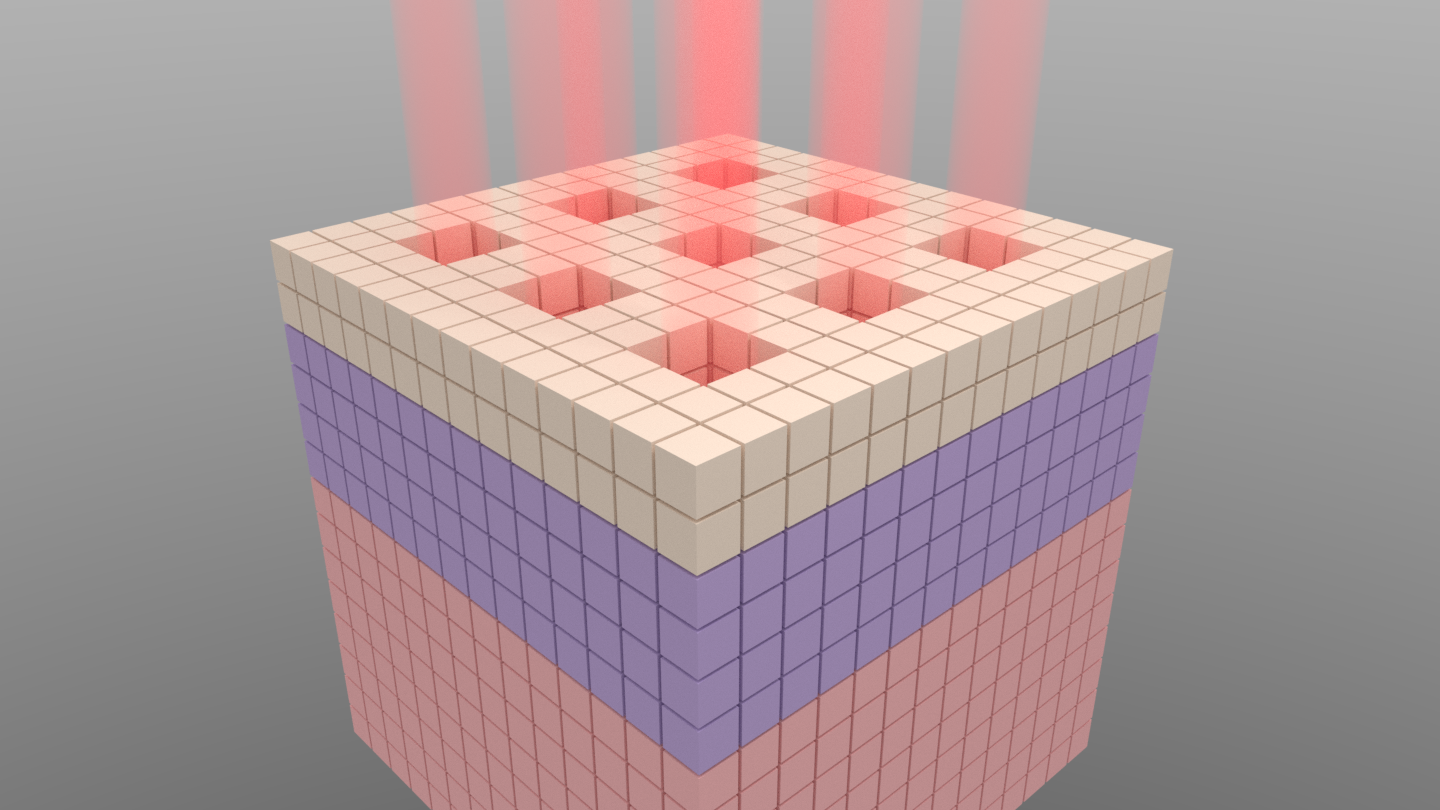
\includegraphics[scale=0.25]{./ablation/images/voxel-model-render.png}
\caption{Example of a possible voxel model, with three different layers, various holes due to ablative pixel beam lasers. Each voxel represents a different optical/thermal propertty of the tissue medium.}\label{fig:voxel-model}
\end{figure}

The original MCRT code was developed for astronomy applications \cite{wood1999model,wood2005estimating}, and has since been adapted for medical applications~\cite{campbell2015monte,barnard2018quantifying}.

\Cref{fig:algo}. shows the overall algorithm for the simulation, including the MCRT portion. 
The MCRT portion of the algorithm begins with determining where the photon enters the medium. This is calculated by randomly selecting one of the pixel beams, from the 9x9 array of pixel beams. Next the position on the surface of the medium is calculated. As the profile of the pixel beams are unknown, they are assumed to be uniformly circular *maybe change to gaussian??*. Thus, the packets position is uniformly sampled on a circle the width of the pixel beam.

Once the packet enters the simulation, a propagation distance for the packets is calculated using \cref{eqn:propdist}. The packet then moves this distance before undergoing an interaction event. This can be either scattering or absorption. This process is repeated until the photon has either been absorbed or exits the medium.

%Equation 1 is for a uniform density (opacity) medium, but you have a grid, so need some description of how you track packets on a grid.


\begin{equation}
L = -\tfrac{ln(\xi)}{\mu_a}
\label{eqn:propdist}
\end{equation}

\noindent Where:\\
\indent $\xi$ a random number ($\tau = -ln(\xi)$, $\tau$ is the optical depth);\\
\indent $\mu_a$ is the absorption coefficient;\\
\indent L is the physical distance.\\

\Cref{eqn:propdist} is the equation for a uniform medium. As the medium we are simulating changes over time due to thermal damage this equation has to be adapted for a 3D Cartesian grid. This is achieved as below:

\begin{equation}

\end{equation}

The above process is repeated until all the photons have been absorbed or have escaped the tissue medium. We use 5 million photons per MCRT simulation run.

\begin{figure}
\centering
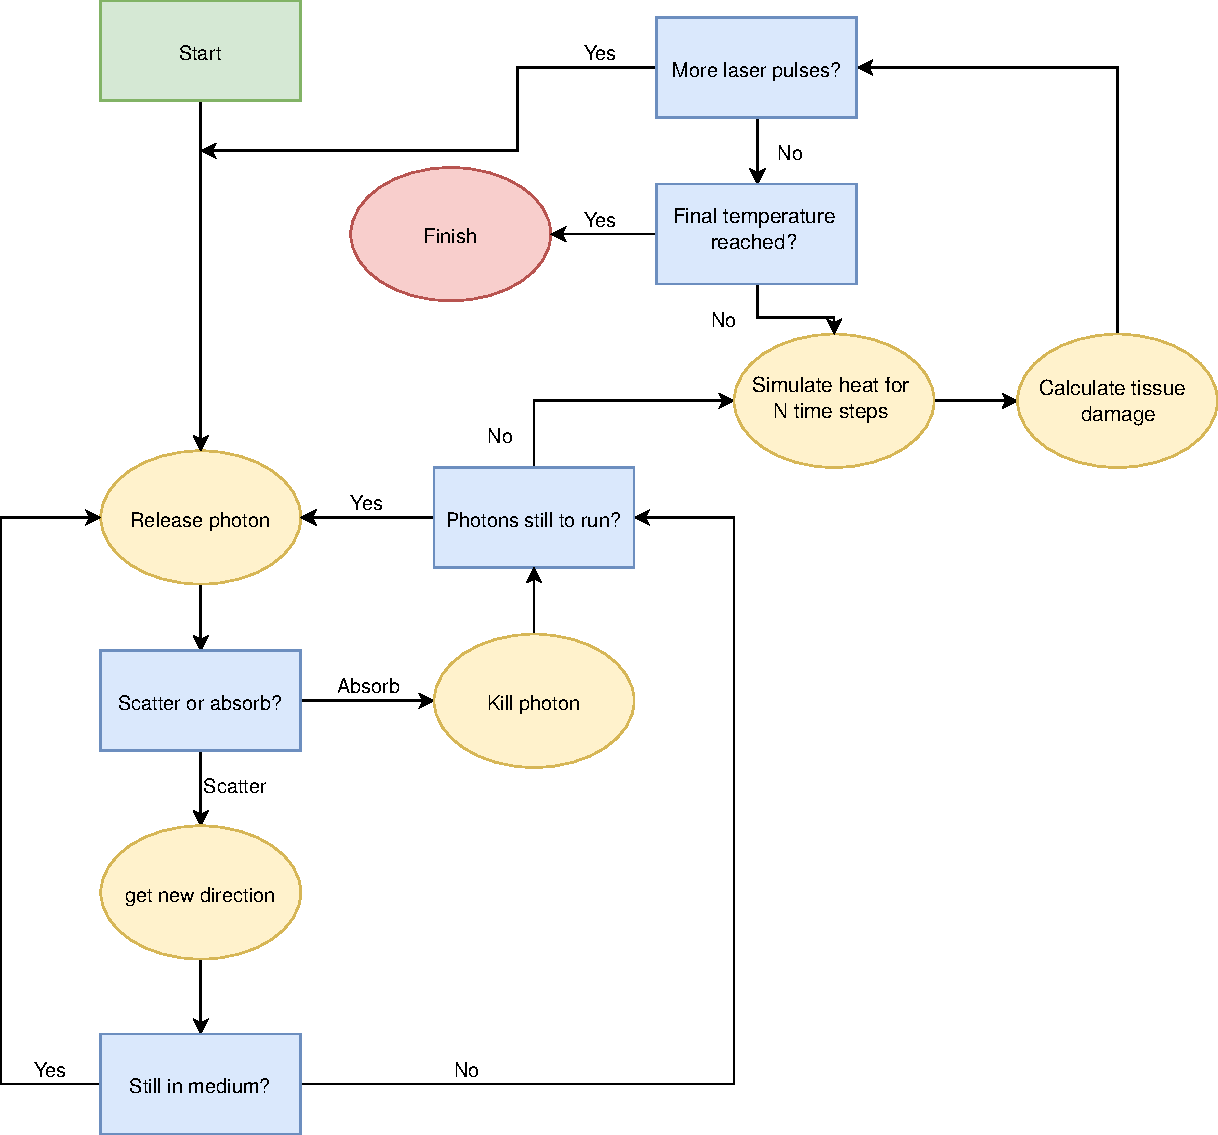
\includegraphics[scale=0.5]{./ablation/images/flowchart.pdf}
\caption{Flowchart of the tissue ablation algorithm.}
\label{fig:algo}
\end{figure}

We calculate the absorbed energy using the path length counter method devised by Lucy \cite{lucy1999computing}. The energy absorbed per voxel is calculated as:

\begin{equation}
E_{i}^{abs} = \frac{L}{N \Delta V_i}\sum\mu_a s
\label{eqn:Eabs}
\end{equation}

\noindent Where:\\ 
	\indent L is luminosity [$W$];\\
	\indent N is the number of photons;\\
	\indent $\Delta V_i$ is the volume of the $i^{th}$ voxel [$m^{-3}$];\\
	\indent $\mu_{a,i}$ is the absorption coefficient of the $i^{th}$ voxel [$cm^{-1}$];\\
	\indent and s is the pathlength of a photon packet through the $i^{th}$ voxel [$cm$].\\
	
\begin{figure}
\centering
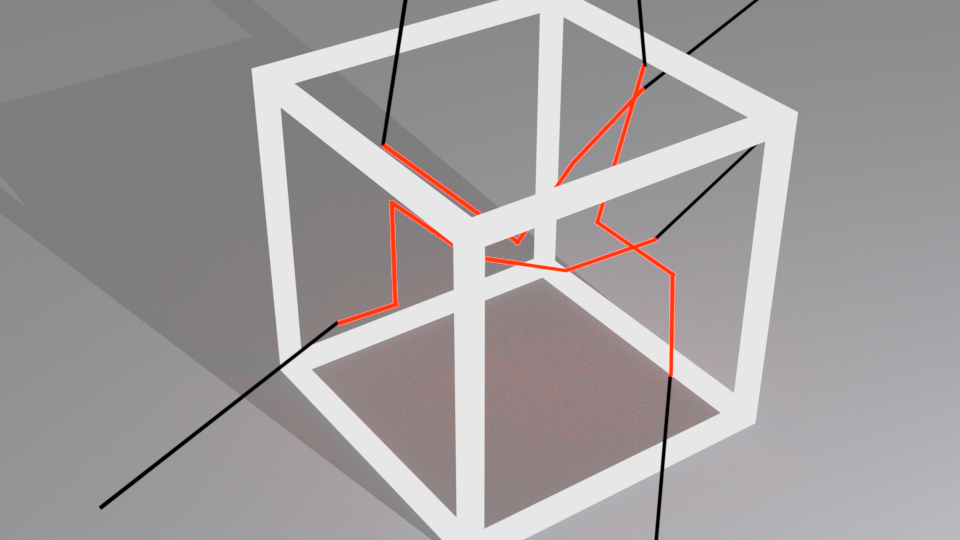
\includegraphics[scale=0.25]{./ablation/images/jmea-explain.png}
\caption{Red lines are photon paths within a voxel. Black lines photon paths outwith the voxel. Red photon paths are summed up in order to calculate the absorbed energy within each voxel.}
\label{fig:jmea-explain}
\end{figure}	
		
This grid of absorbed energy is then passed to the heat transport portion of the simulation.

\subsection{Heat transport}

In order to model the transport of heat in porcine skin, we use the standard parabolic heat equation:

\begin{equation}
\rho c_p \frac{\partial T}{\partial t}= \nabla \cdot (\kappa \nabla T) + \dot{q}
\label{eqn:heat}
\end{equation}

\noindent Where:\\
	\indent $T(x, y, z, t)$ is the temperature as a function of time and space [\textit{K}];\\
	\indent $\kappa$ is the thermal conductivity [$W m^{-1} K^{-1}$];\\ 
	\indent $\rho$ is the density [\textit{Kg}$m^{-3}$];\\
	\indent $c_p$ the specific heat capacity [$J K^{-1}$];\\
	\indent $\dot{q}(x,y,z,t)$ is the source/sink term as a function of time and space [$W m^{-3}$].\\
	
We assume that $\kappa$	is constant during heat transport and only changes between heat transport and MCRT portions of the simulation (see Section Tissue damage), thus:

\begin{equation}
\frac{\partial T}{\partial t}= \alpha \nabla^2 T + \dot{q}
\label{eqn:heatreal}
\end{equation}
	
Where $\alpha = \tfrac{\kappa}{\rho c_p}$ is the thermal diffusivity [$m^2 s^-{1}$]	\\
	
The $\dot{q}$ term is a heat source/sink term. The heat source in this simulation is due to the laser, and we assume the only loss of heat to the surrounding medium is via convection and conduction.
	
These boundary conditions must be considered. All faces of the cube, bar the laser facing face, are considered to be pinned at 5$^{\circ}$C, as the porcine skin was kept cooled prior to experimental work. The laser facing face has a simple convective BC:	

\begin{equation}
\dot{q}_c = -hA(T - T_\infty)
\label{eqn:bceqns}
\end{equation}

\noindent Where:\\
	\indent \textit{h} is the heat transfer coefficient [$W m^{-2} K$];\\
	\indent and \textit{A} is the area of the grid element, that is radiating/convicting heat away [$m^-{2}$].\\

As \cref{eqn:heatreal} is generally hard to solve in arbitrary geometries with complex boundary conditions we employ a numerical method to solve \cref{eqn:heatreal}.
The numerical method we employ in order to solve \cref{eqn:heat} is a the finite difference method (FDM)\cite{ozisik1994finite}. FDM is derived from the Taylor series approximation for derivatives. A function $f(x)$ is discretised onto a grid with \textit{N} nodes (see~\cref{fig:fdmexplain}). Then at node \textit{i} we can use the Taylor series approximation in the forward ($+\text{ive}\ x$ direction) and backward ($-\text{ive}\ x$ direction), and combine the 1$^{st}$ and 2$^{nd}$ derivatives in 1D, where: \textit{i} is the grid point at $x_o$, $i$+1 is the point at $x_0+\Delta x$, and \textit{i}-1 is the grid point at $x_{o}-\Delta x$.

\begin{figure}
  \vspace{-10pt}
  \begin{center}
    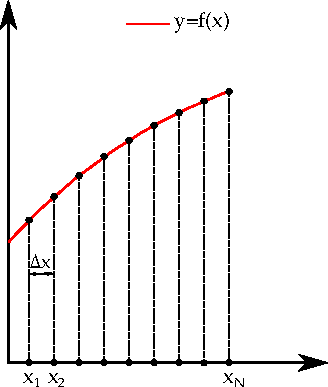
\includegraphics[width=0.48\textwidth]{./ablation/images/fdm.pdf}
  \end{center}
  \caption{Finite difference methods discretisation of \text{f(x).}}\label{fig:fdmexplain}
    \vspace{-20pt}
\end{figure}

\begin{subequations}
\begin{align}
\frac{df}{dx} &= \frac{f_{i+1} - f_{i}}{\Delta x}  &(forward)\\
\frac{df}{dx} &= \frac{f_{i} - f_{i-1}}{\Delta x}  &(backward)\\
\frac{df}{dx} &= \frac{f_{i+1} - f_{i-1}}{2\Delta x}  &(central)\\
\frac{d^2f}{dx^2} &= \frac{f_{i-1}-2f_i+f_{i+1}}{\Delta x^2} &(central)
\end{align}
\end{subequations}


Thus \cref{eqn:heatreal}, in 1D, becomes:

\begin{equation}
T_{i+1}^{n+1} =  \Delta t\alpha \frac{T_{i-1}^n-2T_i^n+T_{i+1}^n}{\Delta x^2} + T_i^n + \dot{q}
\label{eqn:simplefdm}
\end{equation}

\begin{figure}
  \begin{center}
    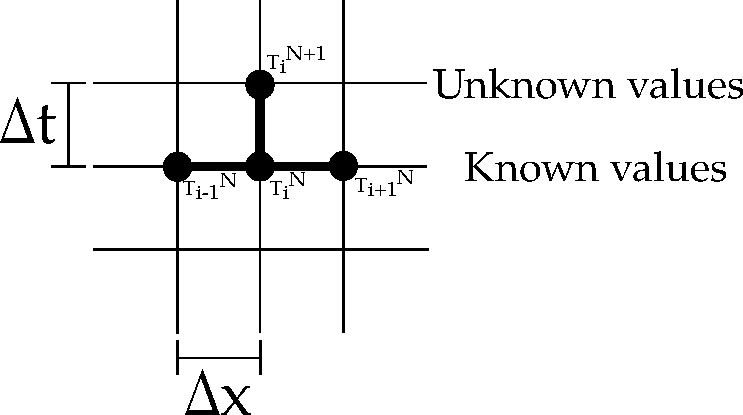
\includegraphics[width=0.48\textwidth]{./ablation/images/fdm-stencil.pdf}
  \end{center}
  \caption{Finite difference method stencil for simple explicit scheme}\label{fig:fdmstencil}
    \vspace{-20pt}
\end{figure}

\Cref{eqn:simplefdm} is called the `simple explicit form of finite-difference approximation'\cite{ozisik1994finite}. \Cref{fig:fdmstencil} shows the `stencil' of this scheme, where there are three known points at time \textit{N}, and just one unknown at time \textit{N+1}. We use a simple explicit scheme here, due to its ease of implementation. This yields for the more general 3D case:


\begin{align*}
U_{xx} &= \frac{\alpha}{\Delta x^2} (T^N_{i-1,j,k} - 2T^N_{i,j,k} + T^N_{i+1,j,k}) \\
U_{yy} &= \frac{\alpha}{\Delta y^2} (T^N_{i,j-1,k} - 2T^N_{i,j,k} + T^N_{i,j+1,k}) \\
U_{zz} &= \frac{\alpha}{\Delta z^2} (T^N_{i,j,k-1} - 2T^N_{i,j,k} + T^N_{i,j,k+1}) \\
T^{N+1}_{i,j,k} &= \Delta t\ (U_{xx} + U_{yy} + U_{zz}) + T^{N}_{i,j,k} + \tfrac{\alpha \Delta t}{\kappa}\dot{q_L}
\label{eqn:FDMheat}
\end{align*}

\noindent Where:\\
	\indent $T^{N+1}_{i,j,k}$ is the new temperature at node $i,j,k$ [$K$];\\
	\indent $T^N_{i,j,k}$ is the temperature at node $i,j,k$ at the current time step [$K$];\\
	\indent $\alpha$ is the thermal diffusivity [$m^2 s^{-1}$];\\
	\indent $\kappa$ is the thermal conductivity [$W/m\cdot K$];\\
	\indent $\Delta x\ etc.$ is the size of the grid element in the $p^{th}$ direction [$m$].\\

Incorporating B.Cs on the top air exposed face:

\begin{equation}
U_{zz} = \tfrac{\alpha}{\Delta z^2} (\tfrac{2 \Delta z}{\kappa} (-h(T^N_{i,j,k}-T^N_\infty) ) -2 T^N_{i,j,k} + 2T^N_{i,j,k+1}) 
\end{equation}

As we are using a simple explicit FDM, the time step is constrained in order to make the solution stable. For a cubic 3D FDM without prescribed flux BCs, yields the constraint: $\Delta t \leq \tfrac{\alpha \Delta x^2}{2\beta}$. However as we have a flux prescribed boundary condition, the constraint on the time is more severe. Along with this time restraint, the pulse length of the laser also has to be considered. If the time step of the heat simulation is too large it will not account for the heat deposited by the laser. Thus, the timestep has to be an order of magnitude smaller than the shortest laser pulse.

As the timestep is small, and the grid resolution large, the resultant simulation is slow. Thus the code has been fully parallelised to improve performance. Both the MCRT and heat simulation are independently parallelised. As MCRT is classed as an `embarrassingly parallel' problem, this portion of the simulation is run on N cores and the results collated and passed to the heat simulation.
The heat simulation is parallelised using a technique called `halo swapping'. This involves splitting up the computational domain, in this case the tissue medium, and separate calculations run on each separate core. They then pass the information from the edge of each of their respective domains to their neighbours (see \cref{fig:haloswap}).


\begin{figure}
\vspace{-45pt}
\centering
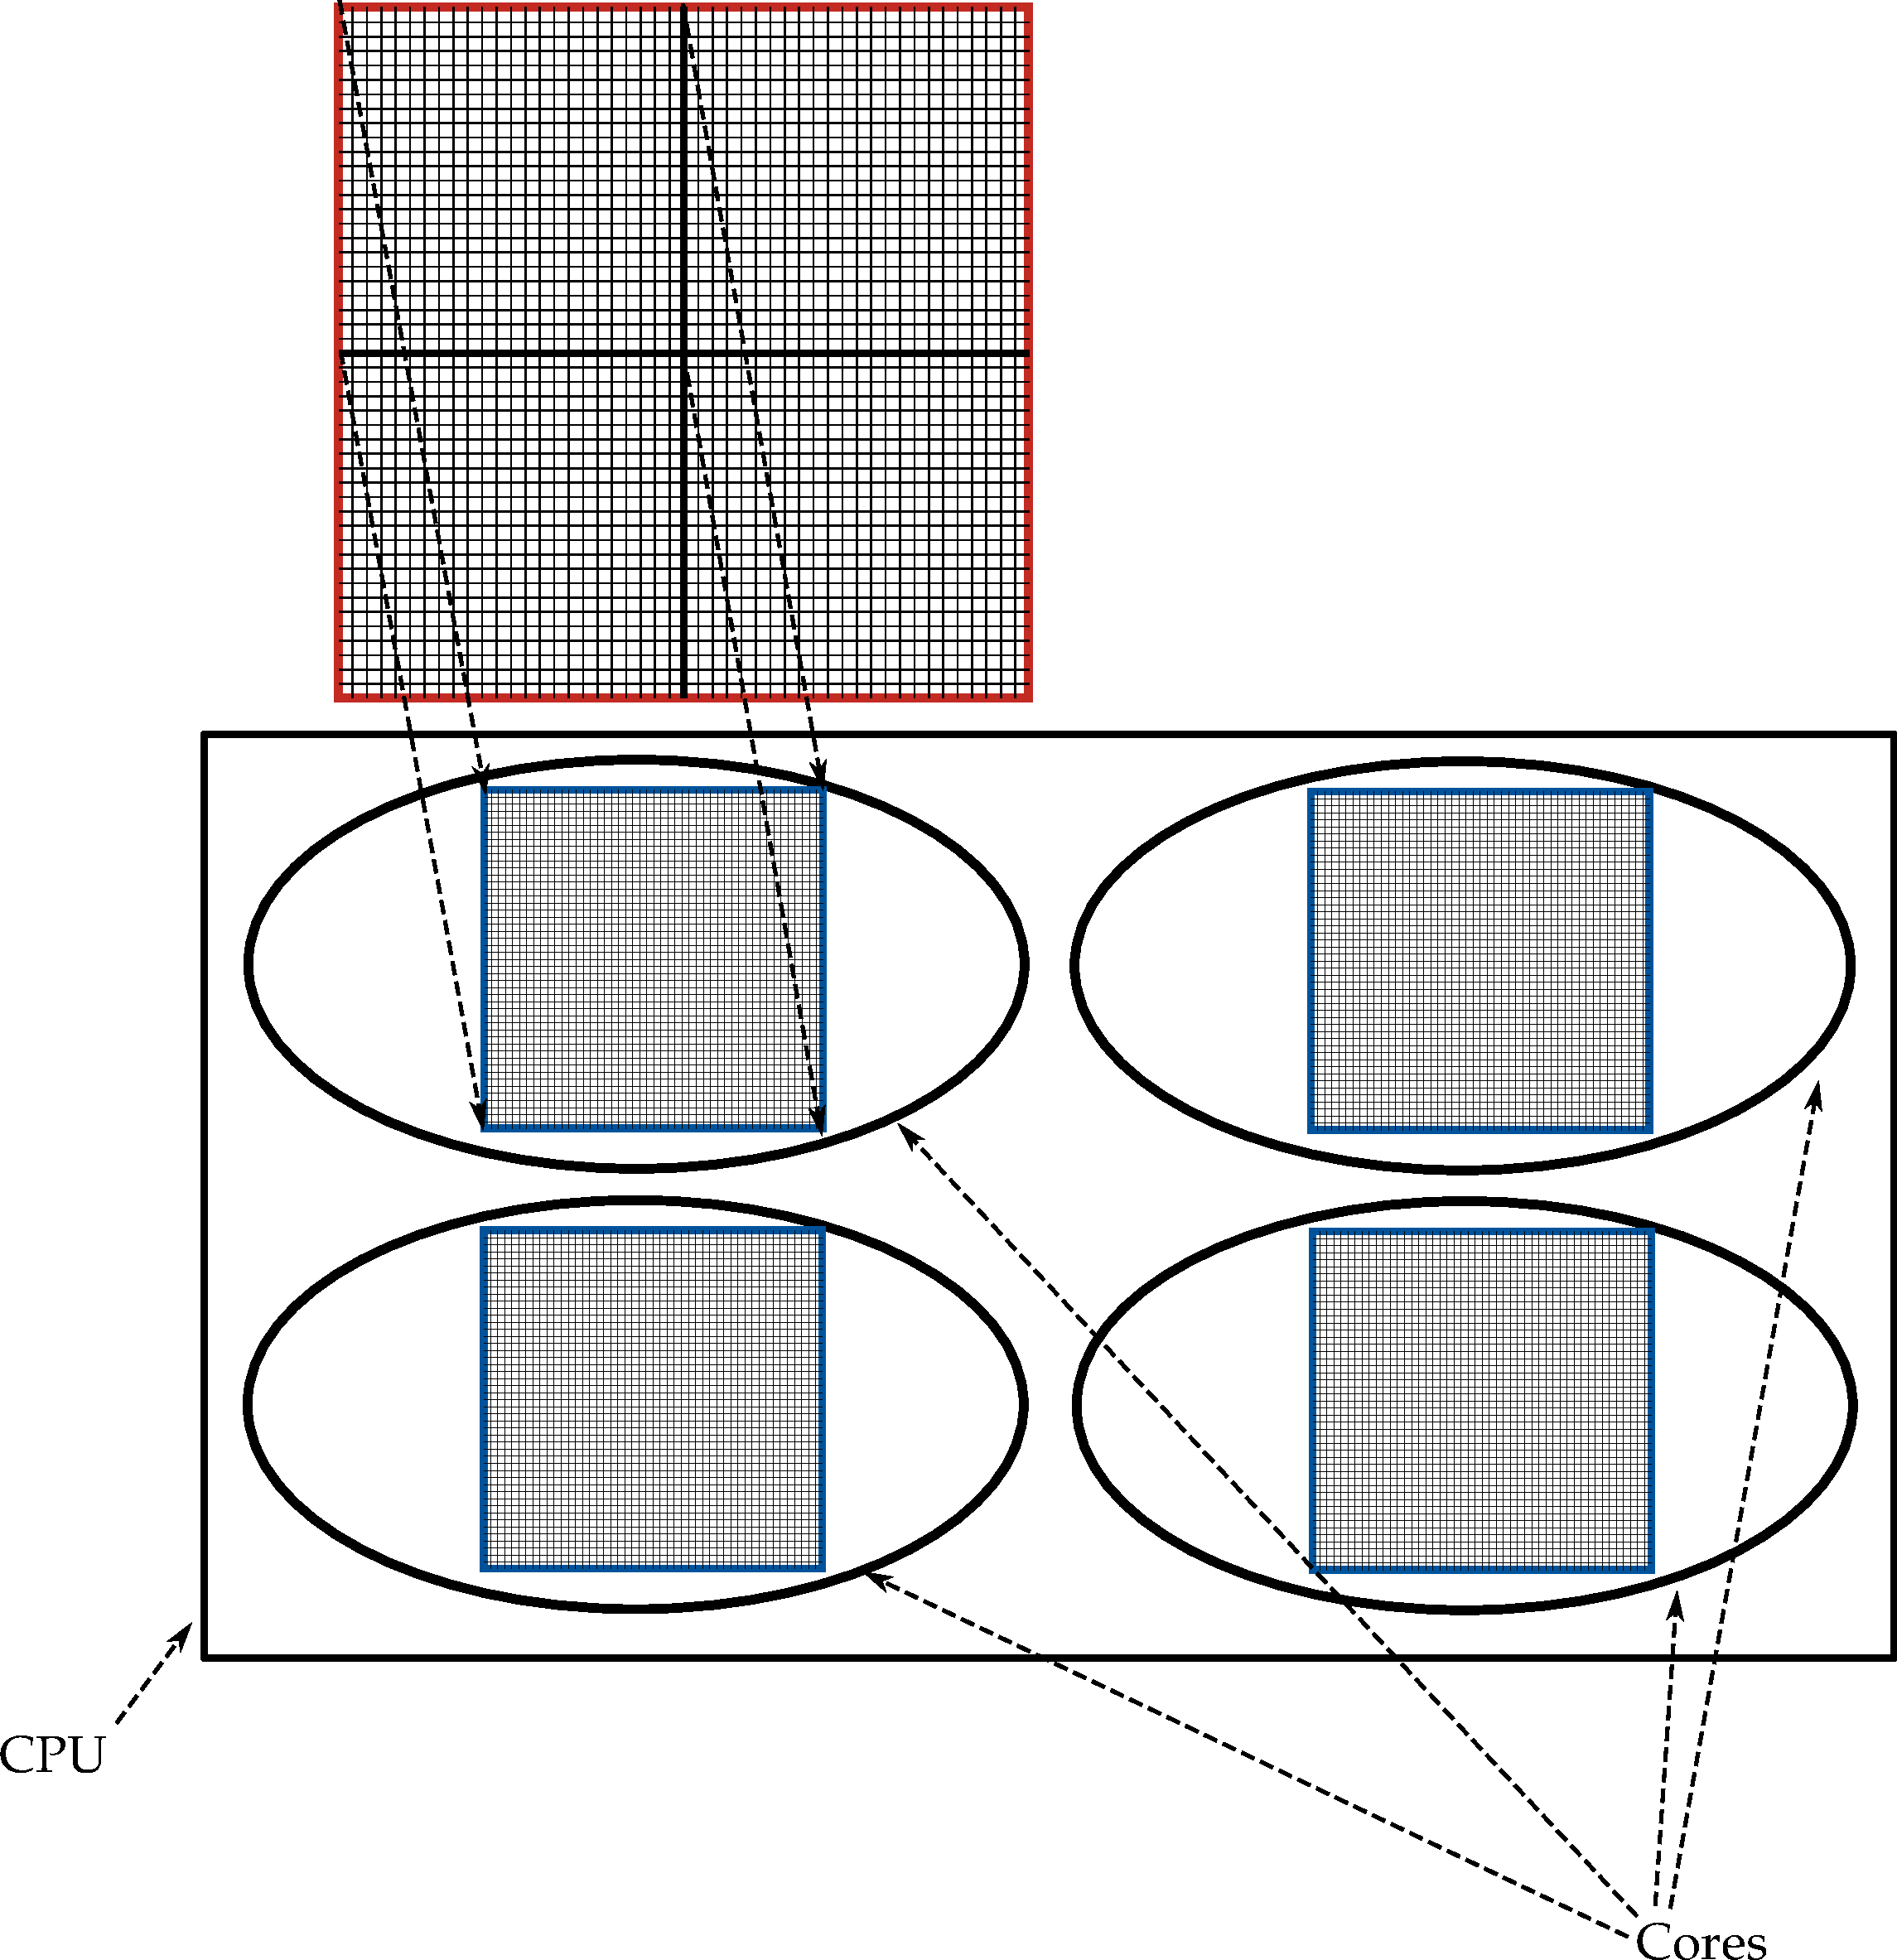
\includegraphics[scale=.35]{./ablation/images/grid-decomp.pdf}
\caption{Computational domain decomposition. Total computational domain is evenly divided between cores in the CPU. This is done via layers of the domain in the z direction. Information is passed to/from cores via the `halo swap' process (see~\cref{fig:haloswap}).}
\label{fig:griddecomp}
\vspace{-10pt}
\end{figure}

\begin{figure}
\centering
\def\svgwidth{350pt}
\input{./ablation/images/halo.pdf_tex}
\caption{Halo swapping. Process A updates the area in red and blue on the left. It updates the blue area which is sent to process B as B's `halo'. Process B cannot update it's own halo, but rather updates the halo for process A.}
\label{fig:haloswap}
\end{figure}


After the heat transport has been completed, the grid of temperatures is passed to the tissue damage portion of the simulation.
\newpage
\subsubsection{Validation of heat transport numerical method}

In order to validate the numerical method we employ to solve the heat equation, we compare the numerical method against an easily solvable case.
Assuming a separable solution in Cartesian for the heat equation yields:

\begin{align*}
T(x,y,z,t)=&(A_1Cos(\alpha x) + A_1Sin(\alpha x))\\
&(B_1Cos(\beta y) + B_1Sin(\beta y))\\
&(C_1Cos(\gamma z) + C_1Sin(\gamma z))e^{-\kappa\mu^2t}\\
\mu^2&=\alpha^2+\beta^2+\gamma^2
\end{align*} 


Then for a cube, side \textit{L}, at $t=0$ the temperature everywhere in the cube is 37$^{\circ}$C. The boundary conditions are:\\

\noindent$T(0,y,z,t)=T(x,0,z,t)=T(x,y,0,t)=0^{\circ}$C\\
$T(L,y,z,t)=T(x,L,z,t)=T(x,y,L,t)=0^{\circ}$C\\

\begin{equation}
\therefore A_1=B_1=C_1=0\
\text{and}\ \alpha=\frac{\pi n}{L}\ \beta=\frac{\pi m}{L}\ \gamma=\frac{\pi p}{L}
\end{equation}

\begin{equation}
T_{nmp}(x,y,z,t)=A_{nmp}Sin\left(\frac{\pi n x}{L}\right)\cdot Sin\left(\frac{\pi m y}{L}\right)\cdot Sin\left(\frac{\pi p z}{L}\right)
\end{equation}

This yields the following solution for the heat equation using the principle of superposition and the boundary conditions:

\begin{equation}
T(x,y,z,t)=\sum^\infty_{n=1,3,..}\sum^\infty_{m=1,3,..}\sum^\infty_{p=1,3,..}\frac{2368}{\pi^3nmp}Sin(\frac{\pi n x}{L})Sin(\frac{\pi m y}{L})Sin(\frac{\pi p z}{L})e^{(-\lambda^2t)}
\end{equation}

\noindent Where:\\
	\indent $\lambda^2=\kappa\pi^2(\tfrac{n^2}{L^2}+\tfrac{m^2}{L^2}+\tfrac{p^2}{L^2})$;\\
	\indent $n,m,p$ are odd integers;\\
	\indent and $L$ is the length of the cube.\\
	
At time, $t=0.1$s, a slice through the middle of the medium yields \cref{fig:validation-heat}.

\begin{figure}	
\vspace{-20pt}
	\centering
	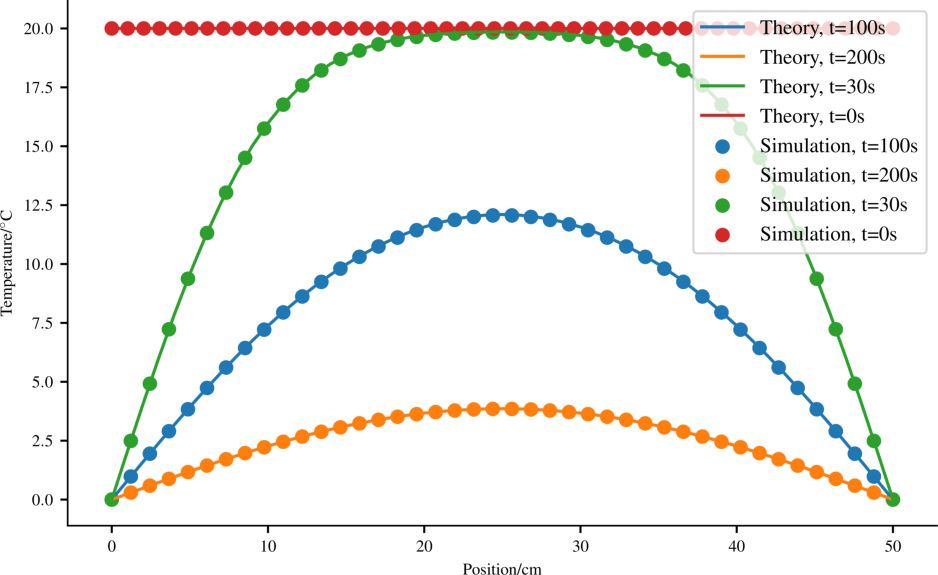
\includegraphics[width=\columnwidth]{./ablation/images/validation.pdf}
	\caption{Comparison between analytical solution and numerical method.}
	\label{fig:validation-heat}
	\vspace{-10pt}
\end{figure}	
	
	
\subsection{Tissue Damage}
\label{sec:tissuedamage}
The final portion of the simulation is the tissue damage model. We use the Arrhenius damage model, originally used as a kinetic model of reaction products in chemistry~\cite{pearce2009relationship}. It has since been adapted by various authors for modelling tissue damage \cite{hendriques1947studies,jiang2002effects}.

\begin{equation}
\Omega(t)=\int^{t_{f}}_{t_i} Ae^{(-\tfrac{\Delta E}{RT})}d\tau
\end{equation}


\noindent Where:\\
	\indent $\Omega$ is the damage value; \\
	\indent A is `frequency factor' [$s^{-1}$];\\
	\indent $\Delta E$ is activation energy [$J/mol$];\\
	\indent R is the universal gas constant [$J mol^{-1} K^{-1}$];\\
	\indent T is the temperature [$K$];\\
	\indent and $t_i$ and $t_f$ are the initial time and final time at $t_{crit}$.\\

It is reported that a value of $\Omega$ of 0.53, 1.0, and 10$^4$ relate to first, second, and third degree burns respectively~\cite{diller1983finite}. We use the Arrhenius damage model in order to better understand the amount of damage caused by the laser in the non-ablated areas of tissue. This can give us an insight into the various physical phenomena encountered in the OCT results.\\

We model tissue damage in four main sections: coagulated, dehydrated, carbonized, and finally ablated sections.\\

Coagulated tissue is the the areas of the tissue where the temperature is above 43$^{\circ}$C, the threshold for damage.
When areas of the tissue reach 100$^{\circ}$C water begins to boil. This acts as a large heat sink for the absorbed laser energy, and is modeled as; 

\begin{equation}
Q_{vaporisation}=M_{voxel} L_{vaporisation}
\label{eqn:latentheat}
\end{equation}

\noindent Where:\\
	\indent $Q_{vaporisation}$ is energy in Joules required to boil off the water in a voxel [$J$];\\
	\indent $M_{voxel}$ is the mass of a voxel [$Kg$];\\
	\indent and $L_{vaporisation}$ is the latent heat of vaporization for water [$J K^{-1}$].\\
	
As water boils off, the water content of each voxel changes. This affects the absorption coefficient, density, thermal conductivity, and heat capacity. Each of these vary linearly with water content per voxel;

\begin{align}
W &= W_{init} - \left(W_{init}*\left(\tfrac{Q_{current}}{Q_{vaporisation}}\right)\right) \\
\rho &= 6.16 \cdot 10^{-5}\ W + 9.38 \cdot 10^{-4} \\
c &= 2.5 \cdot 10^{3}\ W + 1.7\cdot 10^{3} \\
\kappa &= \rho \cdot 10^{-3} (0.454\ W + 0.174)
\end{align}

\noindent Where:\\
\indent $W$ is the water content (i.e W = 0.7 equates to 70\% water content);\\
\indent $W_{init}$ is the initial water content;\\
\indent $Q_{current}$ is the total energy absorbed by the $i^{th}$ voxel since the temperature reached 100$^{\circ}$C;\\
\indent $\kappa$ is the Thermal conductivity [$W m^{-1} K^{-1}$];\\
\indent and c is the heat capacity [$J Kg^{-1} K^{-1}$].\\

We define the ablation temperature ($T_a$) as occurring between 173 and 450$^{\circ}$C\cite{gerstmann1994char}. At the $T_a$ the tissue is removed and set the thermal and density properties to that of air.

The tissue structure is then fed back to the MCRT model and the whole process repeats until the average temperature of the model is under 43$^{\circ}$C. This process is outlined in \cref{fig:algo}.

\section{\textit{In silca} results}
 
\subsubsection{Optical \& thermal properties}

As both of the lasers used in the experimental work are infrared lasers, this means that the optical properties are dominated by water absorption (see \cref{fig:waterabsor}). Er:YAG has a wavelength 2940$~nm$ which corresponds to an absorption coefficient of water: $\sim 11200~cm^{-1}$. The CO$_2$ laser has a wavelength 10.6$~\mu m$ which corresponds to an absorption of coefficient of $\sim 850~cm^{-1}$. As the absorption coefficient is large, we assume that scattering is negligent at these wavelength.
\Cref{table:values} summarises the thermal properties for tissue and air used in the simulations.  

\begin{figure}	
\vspace{-20pt}
	\centering
	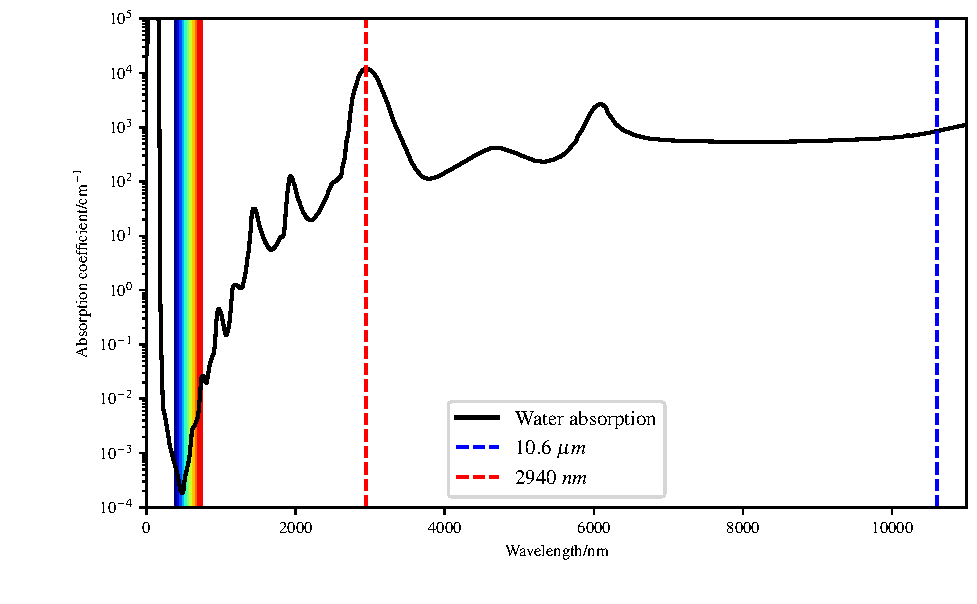
\includegraphics[width=\columnwidth]{./ablation/images/water.pdf}
	\caption{Water absorption coefficient for wavelengths 0-12000nm \cite{segelstein1981complex}. Data shows that water is highly absorbing at large wavelengths.}
	\label{fig:waterabsor}
	\vspace{-10pt}
\end{figure}

\begin{table}
\begin{tabular}{|c|c|c|c|}
\hline 
• & Thermal conductivity, $\kappa$  & Density, $\rho$ & Heat capacity, c \\ 
\hline 
Tissue & $\rho \cdot 10^{-3} (0.454\ W + 0.174)$ & $6.16 \cdot 10^{-5}\ W + 9.38 \cdot 10^{-4}$ & $2.5 \cdot 10^{3}\ W + 1.7\cdot 10^{3}$  \\ 
\hline 
Air & $a e^{-b(T-273.15)} +c$  & $\tfrac{p_{atm}}{R_{spec} T}$ & 1006 \\ 
\hline 
\end{tabular}
\caption{blah blah}\label{table:values}
\end{table}  
 

\subsection{Results}

We model the porcine skin as a cuboid dimensions: 1.1 $\times$ 1.1 $\times$ 0.5 cm. The initial temperature of the porcine skin is assumed to be around 5$^{\circ}$, as the tissue was kept on ice. 
As mentioned in the previous sections, there are several unknowns in the model: $T_a$, water content, temperature of air after ablation. Therefore we run several models so that the full parameter space of these unknowns can be explored.

\subsubsection{Investigating ablation temperature, $T_a$}

Various literature sources report the ablation temperature ranging from 173$^{\circ}$ to 450$^{\circ}$*cite this*. Thus, we run several models over this range. \cref{fig:ta} shows how $T_a$ affects the crater depth as a function of pixel beam energy. At lower pixel beam energies, the tissue ablation temperature has little to no effect on the crater depth. At higher energies, $\geq 125~mJ$, the value of $T_a$ ha a larger effect. For example at $400~mJ$ there is a difference in the crater depth of $\sim0.05~mm$  between the lowest and highest $T_a$.

%Jump straight to fig 9, but would be good to show movie where you see the holes being drilled and medium heating up.


\begin{figure}
	\centering
    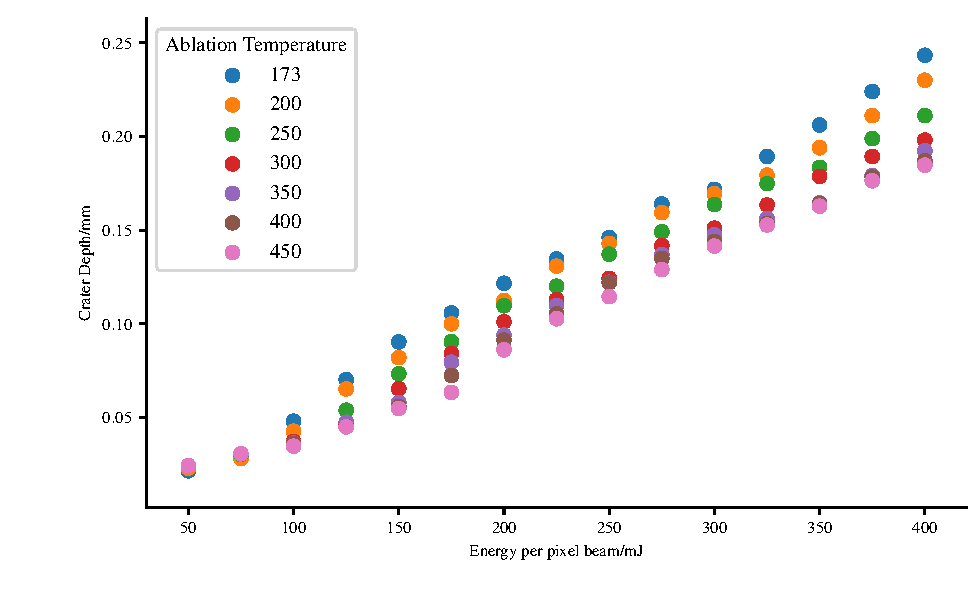
\includegraphics[width=\columnwidth]{./ablation/images/ta.pdf}
    \caption{Simulation of CO$_2$ ablative laser crater depths as a function of pixel beam energy for various $T_a$s.}\label{fig:ta}
\end{figure}
 

\subsubsection*{Investigating water content}
 
\subsubsection*{Investigating temperature of air after ablation} 
 
\section{Conclusion}